\documentclass[letterpaper, 12pt]{article}

\usepackage{geometry}
 \geometry{
 letterpaper,
 total={170mm,257mm},
 left=20mm,
 top=20mm,
 bottom=20mm
 }
\usepackage{graphicx} % Required for inserting images
\usepackage{authblk}
\usepackage{amssymb}
\usepackage{lipsum}
\usepackage{float}
\usepackage{times}
\usepackage{amsmath}
\usepackage[format=plain,
            labelfont={bf,it},
            textfont=it]{caption}
\captionsetup{justification=raggedright,singlelinecheck=false}
\usepackage{ragged2e}
\usepackage{longtable}
\usepackage{comment}
\usepackage{setspace}
\usepackage{fancyhdr}
\usepackage{titlesec}
\usepackage[hyperindex,breaklinks]{hyperref}
\hypersetup{
    colorlinks=true,
    linkcolor=blue,
    filecolor=magenta,      
    urlcolor=blue,
    pdftitle={Overleaf Example},
    pdfpagemode=FullScreen,
    }
% \usepackage{background} % add COSIG logo to page
\usepackage[T1]{fontenc}
\usepackage{helvet}
\renewcommand{\familydefault}{\sfdefault}
\pagenumbering{gobble}
\usepackage[skip=10pt plus1pt, indent=40pt]{parskip}

\begin{comment}
\backgroundsetup{
   scale=1,
   angle=0,
   opacity=1,
   color=black,
   contents={\begin{tikzpicture}[remember picture, overlay]
      \node at ([xshift=3cm,yshift=1cm] current page.south west)
            {
\includegraphics[width = 5cm]{img/home/241017_final_logo_mockup.png}}; %<- change the name of image
     \end{tikzpicture}}
 }
\end{comment}

\titlespacing*{\section}
{0pt}{1.5ex plus 1ex minus .2ex}{1.3ex plus .2ex}

\renewcommand\Authfont{\fontsize{12}{14.4}\selectfont}
\renewcommand\Affilfont{\fontsize{9}{10.8}\itshape}
 
\begin{document}
\flushleft

\includegraphics[width=0.5\textwidth]{img/home/241017_final_logo_mockup.png}

\section*{Misidentified and non-verifiable cell lines}
\textit{Last updated: 5 February 2025}
\subsection*{Cell lines}

A cell line is a population of cells that can be grown in a laboratory culture indefinitely. Cell lines are an essential tool for biomedical research because they allow biological experiments to be performed in vitro (i.e. outside of a living organism). For instance, researchers developing new cancer drugs will certainly test the effect of their drug candidates on many different cancer cell lines before ever considering testing the drug candidate on live animals, let alone human patients.

Because cell lines can grow indefinitely, one research laboratory or laboratory supplier can take a few cells from their cell line stock and give them to another laboratory for that laboratory to begin culturing their own stock. By far the most popular cell line is HeLa, and the many thousands of \href{https://www.cellosaurus.org/CVCL_0030}{HeLa cell stocks} used in biomedical research around the world can all be traced back to the original stock of "immortal" cervical cancer cells taken from \href{https://en.wikipedia.org/wiki/Henrietta_Lacks}{Henrietta Lacks in 1951}.

\subsection*{Misidentified/contaminated cell lines}

One complication of relying on cell lines for biomedical research is that stocks will often become cross-contaminated by other cell lines. For instance, HeLa is extremely aggressive as cancer cell lines go and HeLa cells will easily overtake other cell line stocks that are stored nearby. The popular gastric cancer cell line \href{https://www.cellosaurus.org/CVCL_3360}{BGC-823} is one such victim of HeLa’s aggression; there are no remaining uncontaminated stocks of BGC-823 and thus it is no longer considered an appropriate experimental model for gastric cancer.


\begin{figure}[h!tbp]
    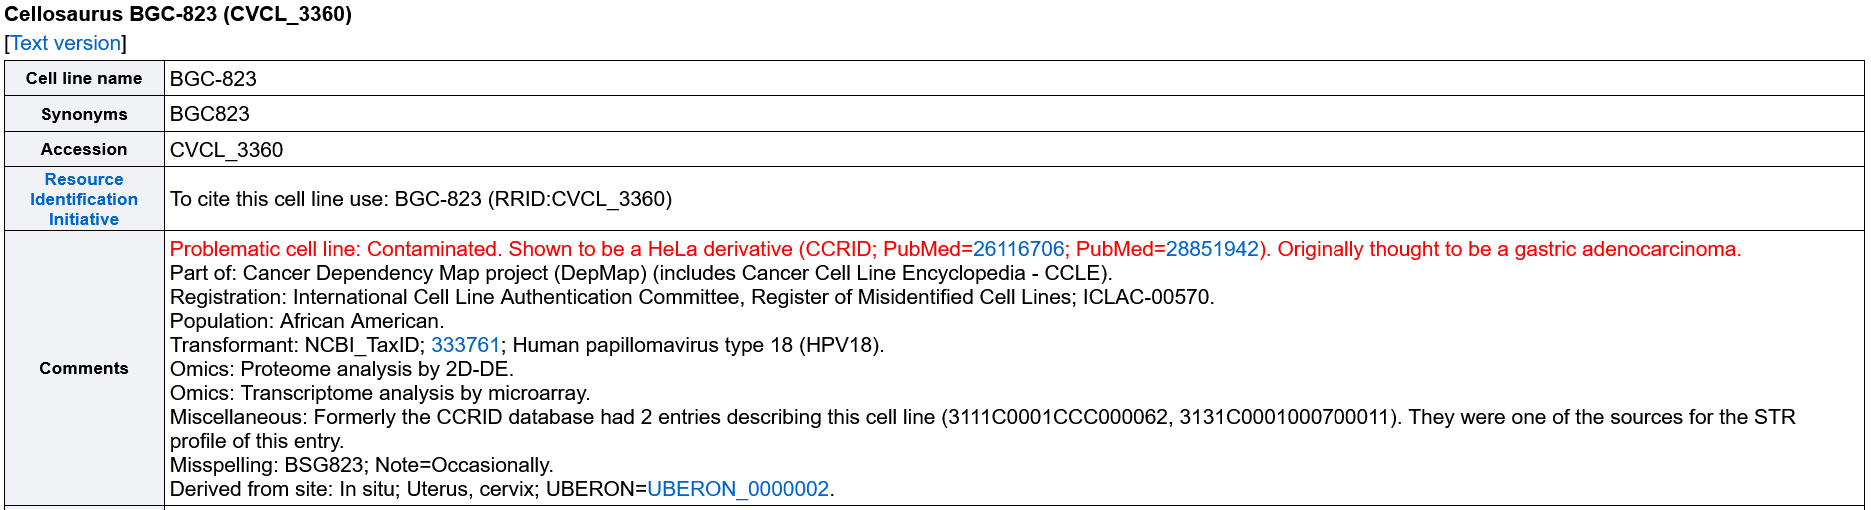
\includegraphics[width=\textwidth]{img/cell_lines/Screenshot 2024-11-04 at 11-59-23 Cellosaurus cell line BGC-823 (CVCL_3360).png}
    \caption*{The Cellosaurus entry for \href{https://www.cellosaurus.org/CVCL_3360}{BGC-823} now warns about the cell line being contaminated by HeLa.}
\end{figure}

The International Cell Line Authentication Committee maintains \href{https://iclac.org/databases/cross-contaminations/}{a register of misidentified cell lines} that is currently 593 entries long. A good number of these cell lines were contaminated by cells from a completely different organism, such as human salivary gland cell line \href{https://www.cellosaurus.org/CVCL_6883}{CAC2}, which is actually made up of unknown cells from a rat.

\href{https://www.cellosaurus.org/index.html}{Cellosaurus} is an encyclopedia of thousands of cell lines and will link to studies showing that a cell line is contaminated or otherwise misidentified.

Because different cell lines can have a wide variety of responses to the same treatment, it is essential that researchers avoid misidentified cell lines and only work with authenticated cell lines that actually represent their system of interest. Consider the fact that cancer cell lines can have wildly different sensitivity to the chemotherapy drug \href{https://www.cancerrxgene.org/compound/Paclitaxel/11/overview/ic50?tissue=PANCANCER&screening_set=GDSC1}{paclitaxel}.

\begin{figure}[h!tbp]
    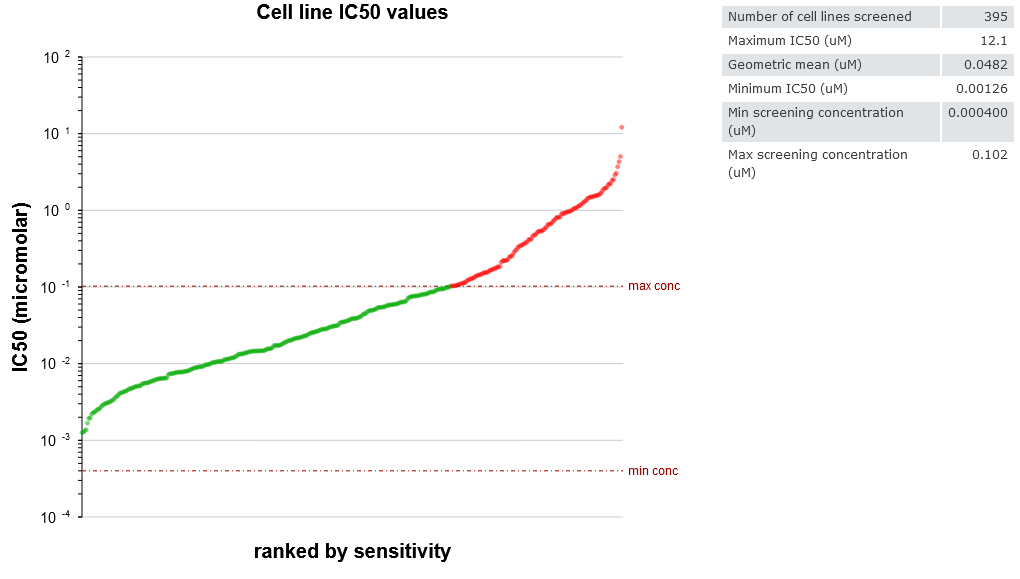
\includegraphics[width=\textwidth]{img/cell_lines/Screenshot 2024-11-04 at 12-02-27 Drug Paclitaxel - Cancerrxgene - Genomics of Drug Sensitivity in Cancer.png}
    \caption*{\href{https://en.wikipedia.org/wiki/IC50}{Half-maximal inhibitory concentration (IC50)}, in this context, is a measure that describes what concentration of a drug is needed to inhibit the growth of a cell line by 50\%. The \href{https://www.cancerrxgene.org/compound/Paclitaxel/11/overview/ic50?tissue=PANCANCER&screening_set=GDSC1}{Genomics of Drug Sensitivity in Cancer (GDSC) database} estimated these values for 395 cell lines for the drug paclitaxel. Note that paclitaxel can be more than a thousand times as potent against some cell lines than others, even for cell lines from the same type of cancer.}
\end{figure}

\subsection*{Cell line verification/authentication}

Researchers should always verify that their cell lines stocks are what they believe them to be. There are a number of ways researchers can verify the integrity of their cell line stocks (many of which are \href{https://www.atcc.org/resources/technical-documents/cell-line-authentication-test-recommendations}{detailed by the American Type Culture Collection}). The most common authentication technique is \href{https://en.wikipedia.org/wiki/STR_analysis}{short tandem repeat (STR) profiling}, which identifies specific molecular signatures in a cell line's genome.

\subsection*{Non-verifiable cell lines}

The names of cell lines are usually just a jumble of letters and numbers and thus can often be easily confused. For instance, the name of \href{https://www.cellosaurus.org/CVCL_3360}{BGC-823} is very similar to that of \href{https://www.cellosaurus.org/CVCL_5334}{MGC-803}, another misidentified gastric cancer cell line. One might easily misspell these cell lines as "BGC-803" or "MGC-823". However, it was recently reported by \href{https://doi.org/10.1002/ijc.34995}{Oste et al. (2024)} that many publications will use these misspelled identifiers to refer to another cell line entirely distinct from these existing cell lines. For instance, \href{https://doi.org/10.1002/jgm.3330}{Zhong et al. (2021)} report experiments in cell lines "BGC-803" and "BSG-823" in addition to experiments in the contaminated cell lines BGC-823 and MGC-803.

Hundreds of articles have referred to experiments in these cell lines despite there being no indication that these cell lines actually exist; there are no entries for these cell lines in any cell line indices, they cannot be found in any supplier catalogs, there are no articles describing how these cell lines were established and no one seems to have produced any genetic profiles of these cell lines to confirm their identities. Oste et al. identified eight such "miscellings": BGC-803, BSG-803, BSG-823, GSE-1, HGC-7901, HGC-803, MGC-823 and TIE-3, although there are certainly many more that have not been studied in detail.

\subsection*{Example 1: Contaminated cell lines}

\href{https://doi.org/10.1016/j.yexcr.2017.09.005}{Liu et al. (2017)} report experiments in the cell lines \href{https://www.cellosaurus.org/CVCL_5334}{MGC-803}, \href{https://www.cellosaurus.org/CVCL_6926}{L02} and \href{https://www.cellosaurus.org/CVCL_0534}{SMMC-7721}. However, each of these cell lines are contaminated by HeLa are thus are no longer considered suitable models for their respective cancers.

\subsection*{Example 2: Non-verifiable and contaminated cell lines}

\href{https://doi.org/10.1186/s12943-018-0874-1}{Yang et al. (2018)} mention and provide experimental results in 10 different cell lines, of which 4 are problematic, shown below in bold:

\begin{itemize}
    \setlength\itemsep{-0.5em}
    \item \textbf{SUN-216}: mentioned once in text of paper and again in Figure 1B, both spelled as SUN-216. SNU-216 is an existing cell line. A possible non-verifiable cell line identifier, but not one that has yet been studied in depth.
    \item \textbf{BGC-823}: Contaminated cell line.
    \item AGS
    \item \textbf{BGC-803}: Mentioned once in text and again in Figure 1B. One of the eight non-verifiable cell line identifiers studied by Oste et al. Likely derived from a typo that confused the cell lines MGC-803 and BGC-823, both contaminated.
    \item NUGC4
    \item MKN74
    \item MKN45
    \item \textbf{SGC-7901}: Contaminated cell line.
    \item HGC-27
    \item GES-1
\end{itemize}

\subsection*{Additional resources}

\begin{itemize}
    \setlength\itemsep{-0.5em}
    \item \href{https://www.atcc.org/resources/technical-documents/cell-line-authentication-test-recommendations}{ATCC Cell Line Authentication Test Recommendations}
    \item \href{https://www.cellosaurus.org/index.html}{Cellosaurus}
    \item \href{https://iclac.org/}{International Cell Line Authentication Committee (ICLAC)}
    \item \href{https://iclac.org/references/reading-reviews/}{ICLAC-curated reviews on cell line misidentification}
    \item \href{https://doi.org/10.1002/ijc.34995}{"Misspellings or 'miscellings'—Non-verifiable and unknown cell lines in cancer research publications" (2024)}

\end{itemize}


\end{document}